\documentclass[10pt]{sugconf-ish}
\usepackage[top=0.75in,bottom=0.875in,left=1in,right=1in]{geometry}
\usepackage{graphicx}

% ----- macro variables used by sugconf -----
\sugconfsubject{NESUG 2007}
\sugconfpapernumber{}
\sugconfkeywords{}


\title{Automated Real-Time Forecasting of Stream Conditions with \SASregistered}
\author{Samuel T. Croker,  Independent Consultant\\
Shane L. Hornibrook,  Independent Consultant \\
Tomonori Ishikawa, USC Department of Statistics, Columbia, SC}
\usepackage[bookmarks=false,
  pdfauthor={\@author},
  pdfcreator={pdfLaTeX sugconf.cls},
  pdfkeywords={\SUGconfKeywords},
  pdfstartview=FitBH,
  pdfsubject={\SUGconfSubject},
  pdftitle={\@title}]{hyperref}

\usepackage{booktabs,nonfloat}
\usepackage{comment,color}


% ----- helpful new commands -----
\newcommand{\degs}{\ensuremath $^{\circ}$}
\newcommand{\mins}{\ensuremath $^{\prime}$}
\newcommand{\secs}{\ensuremath $^{\prime\prime}$}
\newcommand{\isDistr}{\ensuremath $\sim$ }
\newcommand{\xomment}[1]{\textcolor{red}{\textbf{#1}}}


\begin{document}

\begin{abstract}
When you are a \SASregistered\ programmer planning a fishing trip on the Cassleman River in Western Maryland, you want to know what river conditions to expect. One easy-to-run program, incorporating three critical features of SAS, can generate reasonably-accurate, short-term forecasts of river level using real-time data provided online by the United States Geological Survey. First, using the URL access method of the FILENAME statement and basic DATA step techniques, you can import data from the online USGS water data repository. Second, you can analyze the resulting data set and produce forecasts with SAS High-Performance Forecasting procedures by choosing among models as diverse as ARIMA, ESM and UCM. Third, you can display effective graphs of the resulting forecasts with SAS/GRAPH\textsuperscript{\scriptsize\textregistered}. You can easily apply these techniques to other data and analyses to provide a complete SAS-based solution from web-enabled ETL to automatic generation of forecasts to web publication of the results. Keywords: Base SAS, PROC HPFENGINE, PROC HPFARIMASPEC, SAS/GRAPH.
\end{abstract}


\section{Introduction}

As a skilled SAS programmer, you can easily generate accurate forecasts of short-term stream conditions by analyzing river data provided online by the U.S. Geological Survey (USGS). Beginning with web-oriented DATA step techniques, you can import data from online USGS water data repositories. Next, you can produce forecasts using High-Performance Forecasting (HPF) procedures to choose the best model from among a wide range of candidates. Possible models include, but are not limited to, Auto-Regressive Integrated Moving Average (ARIMA) models, Exponential-Smoothing Models (ESM) and Unobserved Components Models (UCM). Finally, you can create attractive figures using SAS/GRAPH, which, to come full-circle, you can post to a website for easy dissemination.

Forecasting stream conditions can be quite challenging given the dizzying array of potential man-made, geophysical and meteorological factors which can influence the behavior of a river's characteristics such as stage and flow. Confronting limited resources of time and effort, you can leverage the power of HPF to evaluate many models for many river data sets in a large-scale forecasting project. However, as any experienced statistician knows, there is simply no substitute for detailed knowledge about the data, and you should not use HPF as a ``black box'' replacement for familiarity with the data.

This paper begins by describing the river data which you can obtain on the web from the USGS. You will see how you can capture and prepare the data. Next, you will read about how to select appropriate forecast models using HPF procedures. Then, you will read about how to use SAS/GRAPH to visualize the forecasts. At the end of the paper, by comparing data from two rivers with contrasting characteristics, you can assess the potential strengths and weaknesses of HPF and review the importance of detailed data knowledge when you select a forecast model.

There are many trout streams in Maryland and Southern Pennsylvania that provide for a great day of fishing.  The allure of Western Maryland is that the more remote location means that there will most likely be fewer lines in the water than in Central Maryland.  If you live in the Washington, DC metro area or in Baltimore, a trip to Western Maryland represents a significant contribution of time and it is more important to know what conditions on the water are before making this commitment.  If conditions on the Casselman River in Western Maryland is not optimal, then you need a few choices in the Central portion of the state to fall back upon. 
The streams shown here are suggested by combining the suggestions made by Gelso and Coburn in Guide to Maryland Trout Fishing and what data is available online, provided by the United States Geological Survey. 

\newpage
Here are the hourly observation profiles for the rivers of study from July 5, 2007 until August 6, 2007.\\


\includegraphics{stage01581920.pdf}Gunpowder Falls near Parkton, MD\\
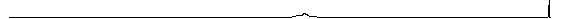
\includegraphics{stage01582000.pdf}Little Falls at Blue Mount, MD\\

\includegraphics{stage01591000.pdf}Patuxent River near Unity, MD\\
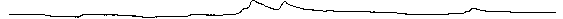
\includegraphics{stage01595000.pdf}North Branch Potomac River at Steyer, MD\\
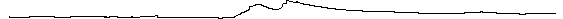
\includegraphics{stage01596500.pdf}Savage River near Barton, MD\\

\includegraphics{stage01597500.pdf}Savage River below Savage River Dam \\
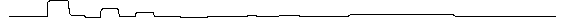
\includegraphics{stage01598500.pdf}North Branch Potomac River at Luke, MD\\
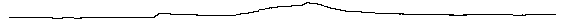
\includegraphics{stage01609000.pdf}Town Creek near Oldtown, MD\\
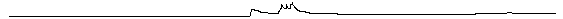
\includegraphics{stage01649150.pdf}Paint Branch Tributary near Colesville, MD\\
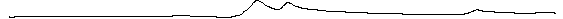
\includegraphics{stage03075500.pdf}Youghiogheny River near Oakland, MD\\
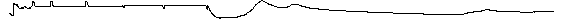
\includegraphics{stage03076500.pdf}Youghiogheny River at Friendsville, MD\\
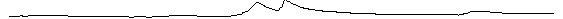
\includegraphics{stage03078000.pdf}Casselman River at Grantsville, MD\\
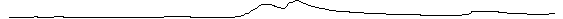
\includegraphics{stage03079000.pdf}Casselman River at Markleton, PA\\



\section{Obtaining and Preparing the River Data}


\subsection{Availability of the Data}
The United States Geological Survey provides a wealth of data online. The USGS reporting system is extensive, and the data layout is fairly complex. Different monitoring stations collect different measurements, but almost all stations collect \emph{stream stage}, the height of the water surface over a fixed point at the station. \emph{Stream flow} is also observed by the USGS at many stations. Fewer stations collect other river characteristics such as water temperature, dissolved oxygen concentration or meteorological data.

Online, the USGS posts river data observations from the most recent 31 days. You would not want to base long-term forecasts on data from such a limited time frame, but you could construct a larger data set which would be more appropriate for long-term forecasting by storing USGS data extracts and appending new observations to the archived data every 31 days.


\subsection{SAS Methods to Retrieve the Data}
You can access the USGS database by pointing-and-clicking from a web browser. However, to extract a large amount of data for a wide variety of stations on demand, you would want to write some type of automating script. While some programmers familiar with web application techniques may use Perl, it is not only possible, but also easy to use SAS to acquire data form the web. This avoids the complexity of marrying the output and input of two scripts and reduces another potential source of maintenance issues.

SAS facilitates hypertext retrieval through LIBNAME statements using the URL library type, also known as the ``LIBNAME URL'' method. Other SAS options include the FILENAME URL method or reading sockets. By reverse engineering the parameters in the USGS URL from a small sample of data requests, you can write a small macro loop to generate DATA step code and import the required data for all USGS stations used in this forecasting project.


\subsection{Guiding Principles for Data Extraction Code Design}

While a detailed examination of the code used to extract the USGS data is beyond the scope of this paper, a guiding principle is readily apparent: design the extraction to gather the data that is available instead of the data that you expect to find. Designing flexibility into your code is the key to success.

Ideally, you would design a data import scheme to examine the river characteristics available at each station and only attempt to import the data that is available at that particular station. Writing such data-driven import code affords flexibility and avoids the necessity of recoding when data availability changes in the source system. You can use the SAS macro language judiciously to generate code based on the data that you actually find instead of simply what you expect to find.

As it happens, the USGS provides reliable data on their websites, both in terms of \emph{data longevity} (it is \emph{where} you expect it to be) and \emph{data quality} (it is \emph{what} you expect it to be). The USGS site provides two core files that facilitate data extraction. First, the USGS lists the locations of the stations where it gathers data. Second, the USGS lists the particular river characteristics (such as temperature, dissolved oxygen, river stage, river flow, etc.) that it gathers at each station.

However, this is not true of many websites. Unfortunately, when ``screen-scraping'' or otherwise pulling data from internet sites, changes in structure, data gaps, and/or periods of unavailability are often the norm, not the exception. Thus, as a general rule, when you design a mechanism to gather data sourced from internet sites, it must be robust enough to gracefully degrade when presented with missing or unavailable data sources.



\subsection{Data Preparation}
The defining characteristic of a \emph{time series} is that it has observations at equally-spaced time intervals. In contrast, \emph{transactional data} occurs at irregular intervals. In this case, 
in order to use time series techniques, the data must be pre-processed. SAS provides several utilities to accomplish this task: the EXPAND, TIMESERIES and HPFENGINE procedures.

PROC EXPAND is the oldest of these procedures and affords the most flexibility in accumulating transactional data to a time series. It can also perform other imputations and transformations that are useful. PROC TIMESERIES can be a little more intuitive for this task. But in the end, PROC HPFENGINE, a component of HPF, can eliminate the need for running multiple procedures. You will note that the analysis in this paper uses the HPFENGINE procedure for data preparation.

An important example of knowing as much as possible about the data is the ability to make distinctions between \emph{structural zeros} and missing values. A structural zero occurs when zero is an actual value for the observation.

To examine this issue in the context of a river stage example, suppose a time series for stream stage has the following observations:
\vspace*{-0.5\baselineskip}
\begin{verbatim}
  3.4 3.6 3.8 . 4.2
\end{verbatim}
\vspace*{-0.5\baselineskip}
In order to proceed with time series analysis, you need to impute the missing fourth observation using the other observations. What value should you use for the missing value?

For stream stage data, if you set the missing value to zero, you would probably be making a mistake. Given the other observations, consider what that would imply about the behavior of the river. Setting the missing value to zero would imply a drop of 3.8 feet from the third observation to the fourth observation of 0 and a rise of 4.2 feet back to the fifth observation. Clearly, you would be wise to use an average interpolation in this situation, perhaps by using a value of 4, the average of the surrounding values of 3.8 and 4.2.

In contrast, suppose you were working with count data or rarely-occurring transactional data. In that case, you could potentially record many missing values if you did not record any observations during the accumulation period. Clearly, you would be wise to use a zero value in this situation since you actually observed no events.

Once again, there is no substitute for familiarity with the data you are analyzing.




\section{Forecast Model Selection and the High Performance Forecasting System}

The SAS High-Performance Forecasting System is an easy-to-use system for evaluating forecast models. With a relatively small amount of code, it is possible to generate forecasts. In fact, it can automatically analyze sample data, chose a holdout-error-minimizing forecast model and output forecasts.

However, you would be foolish to use HPF as ``black box'' forecast generator, substituting its ease-of-use for explicit knowledge about the data and what models might be appropriate. Instead of misusing HPF to make model choices for you in the blind, you should use the power of HPF to augment the number of models that you can evaluate. This way, you can choose a better model by increasing the choice set for your optimal model.


\subsection{Model Class Identification Issues}
There are many books and papers written about time series identification and model fitting, and a thorough discussion of this material is well beyond the scope of this paper, but you should ask yourself several questions when examining data to forecast:
\begin{list}{\textbullet}{\setlength{\itemsep}{0pt}\setlength{\topsep}{0pt}
  \setlength{\parsep}{0pt}}
\item Is the data time series data or is it transactional data?
\item Are short-term or long-term forecasts needed?
\item Does the data exhibit periodicity or seasonality?
\item Are there exogenous variables that may help the forecast if they are included as covariates?   
\end{list}
Your answers to these questions will help determine which models you should evaluate. As with any data-driven forecasting method, the quality of the forecast depends, not only on the data itself, but also on how well you understand and model the data.
%\subsubsection{ARIMA Models}
Auto-Regressive Integrated Moving Average (ARIMA) models are a very flexible class of models that can be very effective at long-term as well as short-term forecasting. However, they can require lots of data for accurate estimation.
%\subsubsection{ES Models}
Exponential Smoothing Models (ESM) can provide very good in-sample, or one-step-ahead, forecasts but often do not perform well in the out-of-sample forecasting region.
%\subsubsection{UC Models}
Unobserved Component Models (UCM) are useful when you know a great deal \emph{a priori} about the structure of the data in terms of seasonalities, cycles and exogenous inputs.


\subsection{Modeling Challenges Posed by River Data}
River data presents unique forecasting challenges. River characteristics can be influenced by a wide range of man-made, geophysical and meteorological factors:
\begin{list}{\textbullet}{\setlength{\itemsep}{0.5\baselineskip}\setlength{\topsep}{0pt}
  \setlength{\parsep}{0pt}}
\item The demand for electricity can influence river stage data recorded downstream from hydroelectric facilities. For example, during hot weather, hydroelectric facilities may release large quantities of water to generate power in order to meet increased demands for air conditioning. In this case, you can observe a square-toothed appearance if you plot the time series for river stage. You can see a strongly seasonal weekday pattern (Monday--Friday has the highest and longest peaks.) due to strong power demand.

\item River stage levels can also affect river flow rates. During times of extremely high or extremely low water levels, river flow can be very different compared to river flow rates when water levels are near median levels.

\item Increasing or decreasing water levels can change the delay parameter when upstream station data is used as an inputs to transfer function models. The amount of this change depends greatly on the shape of the riverbed. Again, if the river spills over its banks, the relationship embodied in a forecasting model can change.
\end{list}


\subsection{How You Should Use HPF in Forecasting River Data}
By now, you should understand how \emph{not} to use HPF, but how is it useful? When can or should you use it? HPF can be an excellent forecasting tool as long as you are using it to augment your knowledge of a time series. If the typical models that forecast the data well for a particular station are known \emph{a priori}, HPF can pick the best one and provide forecasts with little additional input. Thus, HPF can make the chore of forecasting many time series easier by automatically choosing a separate model with the best holdout forecast for each time series. 

For example, if a river station has characteristics that make its data fit several models that are well-known to you, then HPF can easily choose the one that minimizes the holdout error among them. Or, if a river's condition doesn't change much, but you need to update forecasts quite often, HPF can ease the chore of maintaining forecasts.


\section{Visualizing the Results with SAS/GRAPH}

Once you have generated forecasts, you will want to see your results. Visualizing your forecasts is a much more effective than examining a single number metric like Mean Absolute Percentage Error (MAPE). The SAS code below will plot your data and forecasts in three regions: the training sample used to fit the model, the holdout sample used to evaluate an error measure for observed data that you did not use to fit the data and the pure forecasts themselves. 
You can learn more about Sam Croker's \texttt{threeregionforecast} macro in ``Effective Forecast Visualization Using \SASregistered.''

\small
\begin{verbatim}
%macro plotforecast;
  proc sql noprint;
    select count(distinct site_no) into :numsites from &dataset;
    %let numsites=&numsites;
    select site_no
       , max(dtstamp) format=30.
       , min(dtstamp) format=30.
      into 
         :siteno1-:siteno&numsites 
        ,:maxdt1-:maxdt&numsites
        ,:mindt1-:mindt&numsites
      from &dataset 
      group by site_no;
  quit; 
  goptions device=jpeg;
  ods html;
  %do i=1 %to &numsites;    
    %threeregionforecast(outfor(where=(site_no="&&siteno&i"))
      ,&&maxdt&i
      ,&&mindt&
      ,168
      ,168
      ,grtitle="sitename"
      ,dtm=dtstamp    
      ,lciname=lower
      ,uciname=upper
      ,fcname=predict
      ,varname=actual
      ,dtformat=dthour.
      ,xinterval=hour.
      ,xminorticks=0
      ,ymajnum=8
      ,dtdisplay=tod5.
      ,acth=.5
      ,hatitle=""
      ,vatitle="Stage");
  %end;    
  ods html close;
%mend;

%plotforecast;
\end{verbatim}
\normalsize



\section{SAS High-Performance Forecasting for Stream Conditions}

\subsection{Forecasting the Ashley River with HPF: A Little Knowledge Goes a Long Way}
The historic city of Charleston, SC is situated on a peninsula that lies between the Ashley River to the west and the Cooper River to the east. In fact, Charlestonians have a saying that the Ashley and Cooper Rivers meet in Charleston to form the Atlantic Ocean.

\begin{minipage}{\linewidth} 
\centering
\includegraphics[width=6in,keepaspectratio]{AshleyData.jpg} 
\figcaption{River Stage for USGS Station 02172081: Ashley River Near North Charleston, SC}
\label{fig:Ashley}
\end{minipage} 

As you can see in Figure \ref{fig:Ashley}, the river stage of the Ashley River at USGS station 02172081 is greatly influenced by tides. Tidal cycles are composed of a set of well-known, very regular cycles. If you incorporate them into a structural model, you can dramatically improve the forecast. Figure \ref{fig:Ashley} displays hourly observations of river stage from July 5th, 2007 to July 19th, 2007. You can see a clear sinusoidal pattern in the river stage time series driven by the tides.

But, suppose you ignore the tidal information and simply feed the series into HPF, misusing HPFDIAGNOSE by giving it no other information. How good a forecast do you think HPF will produce? The offending code below is deceptively compact:

\small
\begin{verbatim}
proc hpfdiag
  data=WORK.SC_rivers
  print=all
  repository=WORK.arima 
  criterion=aic
  outest=diagest;
    by site_no;
    id dtstamp interval=hour accumulate=avg;
    forecast stage;
    ucm component=(all);
    arimax outlier=(detect=maybe) method=minic;
    esm;
    idm;
    trend dif=auto;
    transform type=auto;
run;
\end{verbatim}
\normalsize

You can see the result in Figure \ref{fig:Ashley_HPF_naive}. HPF choose a relatively simple ARIMA model which has poorer results than you might expect: the amplitude of the forecast is quickly attenuated to the mean in the forecast period.

\begin{minipage}{\linewidth} 
\centering
\includegraphics[width=6in,keepaspectratio]{AshleyArima.jpg} 
\figcaption{Naive HPFDIAGNOSE Forecast (ARIMA) for the River Stage of the Ashley River}
\label{fig:Ashley_HPF_naive}
\end{minipage} 

But HPF can do considerably better if you use a bit of research on tidal cycles. You can examine the period of the primary tidal component cycles at a website maintained by the Oak Ridge National Laboratory:

\hspace*{2em}\url{http://www.phy.ornl.gov/csep/CSEP/OM/NODE31.html}

Using this little bit of information about the tides dramatically improves the forecast. Once again, the SAS HPF code to exploit this information is very compact:

\small
\begin{verbatim}
proc hpfucmspec 
    repository=WORK.arima
    label="Tidal Structural Model"
    name=UCMTIDAL;
  forecast symbol=stage;
  irregular;
  level;
  cycle period=12.42;
  cycle period=12.00;
  cycle period=24.06;
run;
\end{verbatim}
\normalsize

Figure \ref{fig:Ashley_UCM_Tidal} illustrates the improvements.

\begin{minipage}{\linewidth} 
\centering
\includegraphics[width=6in,keepaspectratio]{AshleyStructural.jpg} 
\figcaption{River Stage of the Ashley River: Forced UCM Tidal Model}
\label{fig:Ashley_UCM_Tidal}
\end{minipage} 


\newpage
\subsection{Using HPF to Determine Where to Fish}
As you can see, depending upon the river, forecasting conditions can be tricky. You need local knowledge of what the stage values mean regarding the conditions on the river.  

For a fishing trip in Western Maryland, you would be interested in if there is enough water to fish, or if conditions are unsafe for wading.  With a dashboard application designed from this data you can have much of this information presented in one place so that you can make an informed decision. Other data that should be included could be filled in with local knowledge of the streams themselves and local weather reports.

%\subsection{Model Preparation}
In this example, you would properly use the HPFDIAGNOSE procedure to suggest alternative forecast models, but not rely upon it exclusively for model selection. If you have developed a familiarity with these  rivers, you would have performed some preliminary time series analysis and identified classes of ARIMA and cyclic UCM models as appropriate models. For example, using your knowledge of one of these rivers, you might generate ARIMA models using the PROC HPFARIMASPEC with P(0..3) Q(0..3) and D(0,1,7). By adding the models suggested by HPFDIAGNOSE to your set of model candidates, you are wisely using HPFDIAGNOSE as a check to see if you have missed any simple models that provide reasonably good forecasts.

You would make the identified models available to HPF using several procedures. The HPFARIMASPEC, HPFESMSPEC and HPFUCMSPEC procedures build the specifications for different models, and the HPFSELECT procedure gathers them into a model selection list. Here, the HPFDIAGNOSE procedure attempts to find the best model without regard to known series information. 

%\section{Let's Go Fishing!}
You would accomplish the forecasting itself, as well as accumulation of the time-stamped data, using the HPFENGINE procedure.

\small
\begin{verbatim}
proc hpfengine 
    repository=work.arima
    globalselection=myselect
    data=MARYLAND
    outfor=outfor
    outest=outest 
    back=24
    lead=48
    print=(select);
  by site_no;
  id dtstamp 
    interval=hour 
    accumulate=avg;
  forecast stage;
run;
\end{verbatim}
\normalsize

You can see the results for forecasting river stage on the Cassleman River near Grantsville, MD in Figure \ref{fig:Cassleman}. This graph shows the fit, holdout and forecast periods.

These graphs show both the holdout and the forecast period for all of the stations in the set of rivers that are being analyzed. It is clear that you can probably expect no dramatic changes within the next 48 hours so plans can be made accordingly. All that is left to do is pack up and head to the water! 

\begin{minipage}{\linewidth} 
\centering
\includegraphics[width=6in,keepaspectratio]{cassleman.jpg} 
\figcaption{Cassleman River Near Grantsville, MD August 5th--6th, 2007}
\label{fig:Cassleman}
\end{minipage}

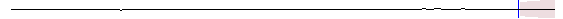
\includegraphics{fc01581920.pdf}Gunpowder Falls near Parkton, MD\\
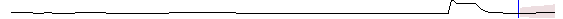
\includegraphics{fc01582000.pdf}Little Falls at Blue Mount, MD\\
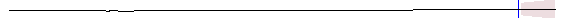
\includegraphics{fc01591000.pdf}Patuxent River near Unity, MD\\
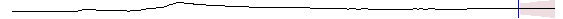
\includegraphics{fc01595000.pdf}North Branch Potomac River at Steyer, MD\\
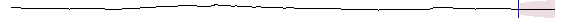
\includegraphics{fc01596500.pdf}Savage River near Barton, MD\\
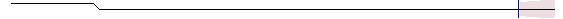
\includegraphics{fc01597500.pdf}Savage River below Savage River Dam \\
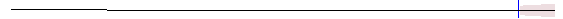
\includegraphics{fc01598500.pdf}North Branch Potomac River at Luke, MD\\
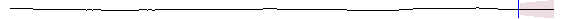
\includegraphics{fc01609000.pdf}Town Creek near Oldtown, MD\\
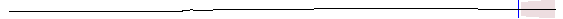
\includegraphics{fc01649150.pdf}Paint Branch Tributary near Colesville, MD\\
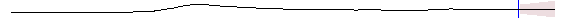
\includegraphics{fc03075500.pdf}Youghiogheny River near Oakland, MD\\
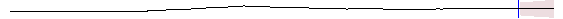
\includegraphics{fc03076500.pdf}Youghiogheny River at Friendsville, MD\\
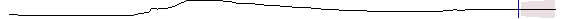
\includegraphics{fc03078000.pdf}Casselman River at Grantsville, MD\\
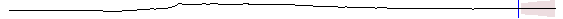
\includegraphics{fc03079000.pdf}Casselman River at Markleton, PA\\

So for August 8, 2007 the Casselman River might be a great place to fish.  You might want to take other issues not covered in this analysis into account.  The grey bands are an arbitrary ``comfort zone'' that signifies the ideal conditions on the water.  These are simply the deviation of the mean of the entire series and do not really correspond to reality.  Local knowledge is required to set these bands accurately and they may differ from person to person as well.  You might choose any of these streams that have comfortable conditions. 

\section{Conclusion}
The targeted rivers in this analysis are pretty stable rivers.  Observations of their river stage reveal characteristics of a regular, long-memory time series.  This makes them excellent candidiates for forecasting using the SAS High-Performance Forecasting porcedures.  In fact, owing to the stability of the river stage, you can even generate relatively good forecasts with little detailed knowledge of the data.  However, you would be unwise to attempt a similar blind forecast of the Ashley River.  The river stage of the Ashley exhibits strong tidal influences.  You can obtain superior forecasts by incorporating some konwledge of tidal cycles.  Thus the statisitcian's exhortation to know as much as possible about the data holds true: you can leverage your knowledge to generate better forecasts. 

SAS HPF provides excellent tools that can leverage detailed knowledge of the data to aid in maintaining or updating forecasts for a large-scale project when the domain of possible models is well-understood. It is also possible to use HPF in an exploratory data analysis role. However, you would be unwise to attempt a similar blind forecast of the Ashley River. The river stage of the Ashley exhibits strong tidal influences. You can obtain superior forecasts by incorporating some knowledge of tidal cycles. Thus, the statistician's exhortation to know as much as possible about the data holds true: you can leverage your knowledge to generate better forecasts. 

SAS HPF provides excellent tools that can leverage detailed knowledge of the data to aid in maintaining or updating forecasts for a large-scale project when the domain of possible models is well-understood. It is also possible to use HPF in an exploratory data analysis role.

Any forecasting system subordinates model fitting because forecasts are typically judged only on holdout error performance. When you need forecasts of rivers that are strongly-influenced by man-made, geophysical or meteorological factors, a model fitting approach that incorporates such exogenous factors may be a superior approach. SAS provides many good options for model fitting as well as forecasting.

If you need an automated forecasting system relying on data from an online data repository, you can easily construct an all-SAS-based solution from data extraction to forecast generation to forecast visualization using the SAS DATA step, SAS High-Performance Forecasting and SAS/GRAPH.




\section{References}

\begin{list}{}{\setlength{\leftmargin}{2em}\setlength{\itemindent}{0em}\raggedright}
\item Box, George E.P., Gwilym M. Jenkins and Gregory C. Reinsel. 1994. 
\emph{Time Series Analysis: Forecasting and Control}, 3rd ed. Upper Saddle River, NJ: Prentice-Hall.

\item Brocklebank, John and David A. Dickey. 2003. 
\emph{\SASregistered\ for Forecasting Time Series}, 2nd ed. Cary, NC: SAS Institute Inc.

\item Gelso, Charlie, Larry Coburn. 2006. \emph{Guide to Maryland Trout Fishing:  The Catch and Release Streams} Carter, OK: Falling Star Publishing

\item Cartier, Jeff. ``The Power of the Graphics Template Language.'' \emph{Proceedings of the 30th Annual \SASregistered\ Users Group International Conference}. April 2004. %\\
$<$\url{http://support.sas.com/rnd/datavisualization/papers/sugi30/GTL.pdf}$>$ (Accessed July 18, 2007).

\item Croker, Samuel T. ``Effective Forecast Visualization with SAS/GRAPH.'' \emph{SAS Global Forum 2007 Proceedings}. April 2007. \\ $<$\url{http://www8.sas.com/scholars/Proceedings/2006/DataPresentation/DP01_06.PDF}$>$

\item Shumway, Robert H. and David S. Stoffer. 2006. 
\emph{Time Series Analysis and Its Applications with R Examples}, 2nd ed. New York: Springer Science+Business Media, LLC.
\end{list}




%\section{Acknowledgments}



\newpage
\section{Contact Information}
We value and encourage your comments and questions! You can find the latest version of the SAS code for this paper at: \url{http://www.scoyote.net/forecasting/}. Please note that we may update this code for use in other papers.

You can contact the authors at:

\begin{tabular}[t]{rl}
\textbf{Name:} & Samuel T. Croker \\
%\textbf{Address:} & Kyzer Rd \\
% & Lexington, SC 29073 \\
%Work Phone:        & 803-240-2805 \\
%Fax:               & 987-654-3210                     \\
%\textbf{E-Mail:} & \href{scoyote@scoyote.net?subject=SESUG 2007 Paper Question}
%{\texttt{scoyote@scoyote.net}} \\
\textbf{E-Mail:} & \texttt{scoyote at scoyote.net} \\
\textbf{Web:} & \url{http://www.scoyote.net/forecasting/} \\
 & \\
\textbf{Name:} & Shane L. Hornibrook \\
%\textbf{Address:} &  \\
% & Davenport, FL \\
%Work Phone:        & 987-654-1234                     \\
%Fax:               & 987-654-3210                     \\
\textbf{E-Mail:} & \texttt{sesug\_paper at shanehornibrook.com} \\
%Web:               & mycompany.com                    \\
 & \\
\textbf{Name:} & Tomonori Ishikawa \\
%\textbf{Address:} & PO Box 211589 \\
% & Columbia, SC 29221-6578 \\
\textbf{E-Mail:} & \texttt{ish at alum.mit.edu} \\
\textbf{Web:} & \url{http://www.stat.sc.edu/~ishikawa/} \\
\end{tabular}


\vfill
% ----- macro variables used by sugconf -----
\SASisRegisteredTrademark\ \OtherTrademarks


\end{document}
